%
% ****
\chapter{Performance \& Auswertung}
\label{chap:erg}
% ****
%
	Ziel dieser Arbeit war es, auf Grundlage eines bereits bestehenden, neuronalen Netzes eine Anwendung des Reinforcement Learning zur Regelung dynamischer Systeme zu schaffen. Das neuronale Netz ist dabei kein konventionell erzeugtes Netz einer künstlichen Intelligenz, sondern beruht auf biologischen Forschungsergebnissen echter Lebensformen.\\
	Somit wurde zuerst eine Berechnungsgrundlage eines solchen Netzes geschaffen und implementiert. Dazu wurden verschiedene numerische Lösungsverfahren von Differentialgleichungen verglichen und umgesetzt. Letztlich wird ein universeller Simulator geschaffen, welcher Informationen über die Nervenzellen und Synapsen erhält und entsprechend in der Lage ist, das gesamte Netz zu simulieren und Fire-Events auszugeben. Um die Performance des neuronalen Netzes durch den Simulator zu messen, wird eine Simulationsumgebung eingebunden und ein Lern-Algorithmus implementiert. In dieser Arbeit wird sich auf die Reinforcement Learning Methode RandomSearch konzentriert sowie auf die Optimierungsmethode durch Gewichten der entsprechenden Synapsen.

% ***
\section{Performance implementierter Algorithmen}
\label{sec:erg_performance}
% ***
	Schnelligkeit der Ausführung von Algorithmen und ganzen Skripten ist in dieser Anwendung von großer Relevanz. Da der Simulator von Grund auf darauf ausgerichtet wurde, später rechenintensive Simulationen von Parametern zu durchlaufen, wurde bereits in der Auswahl der zusätzlich genutzten Pakete darauf geachtet, dass diese performant und vorzugsweise direkt in \texttt{C} implementiert wurden.\\
	Angefangen bei den Berechnungsmodulen in der Datei \texttt{lif.py} wird für komplexere mathematische Operationen die Erweiterung \texttt{NumPy} aus dem bekannten Python-Paket \texttt{SciPy} genutzt. Weiterhin werden Schleifen und If-Abfragen ohne Redundanzen und unnötige Befehle implementiert, um in der höheren Abstraktionsebene einen einwandfreien Aufruf zu garantieren. Nach erfolgreichen Tests der implementierten Funktionen wurde das Framework für den Simulator erstellt. Genutzte Pakete wie \texttt{matplotlib} oder \texttt{hickle} sind ebenfalls für ihre Schnelligkeit und einfache Handhabung ausgewählt worden. Des Weiteren können hier die bereits implementierten Funktionen zur Berechnung von Synapsenströmen und Membranpotentialen einfach importiert werden.\\
	Letztendlich ist die Ausführung des Suchalgorithmus RandomSearch sowie des Optimierers Weights ausschlaggebend. Diese Algorithmen wurden im Laufe der Implementierung immer wieder optimiert und verbessert, sodass eine zuverlässige Simulation mit effizienten Laufzeiten möglich wird. Bei festen Simulationszeiten werden auf der bereits vorgestellten virtuellen Instanz folgende Ergebnisse erzielt (Stichprobenartig aufgelistet).
	\begin{table}[htb]
		\centering
		\resizebox{0.6\columnwidth}{!}{%
		\begin{tabular}{c@{\hskip 0.5cm}c@{\hskip 0.5cm}c@{\hskip 0.5cm}c}    \toprule
			\setlength{\tabcolsep}{50pt}
			\renewcommand{\arraystretch}{1.5}
			\emph{Zeitstempel}	& \emph{Reward} 	& \emph{Laufzeit}	& \emph{Anz. Simulationen} 	\\\midrule
			20180815\_10-40-23  & 26				& 2 Std.			& $39.006$					\\ 
			20180816\_01-50-01	& 123				& 12 Std.			& $10.509.904$				\\
			20180816\_01-52-01	& 185				& 12 Std.			& $10.536.512$				\\
			20180818\_02-48-01	& \textbf{200}		& 12 Std.			& $10.852.326$				\\\bottomrule
			\hline
		\end{tabular}}
	\caption{Parametersuche durch Algorithmus \texttt{RandomSearch}.}
	\label{tab:sim_rs}
	\end{table}
	\begin{table}[htb]
		\centering
		\resizebox{0.6\columnwidth}{!}{%
		\begin{tabular}{c@{\hskip 0.5cm}c@{\hskip 0.5cm}c@{\hskip 0.5cm}c}    \toprule
			\setlength{\tabcolsep}{50pt}
			\renewcommand{\arraystretch}{1.5}
			\emph{Zeitstempel}	& \emph{Reward} 	& \emph{Laufzeit}	& \emph{Anz. Simulationen} 	\\\midrule
			20180815\_11-21-46  & 56				& 1 Std.			& $5.927$					\\ 
			20180816\_13-50-01	& 149				& 12 Std.			& $3.715.008$				\\
			20180816\_13-52-01	& \textbf{200}		& 12 Std.			& $3.686.723$				\\
			20180818\_...		& \textbf{200}		& 12 Std.			& $123.$					\\\bottomrule
			\hline
		\end{tabular}}
		\caption{Optimierung durch Algorithmus \texttt{Weights}.}
		\label{tab:sim_weights}
	\end{table}
	Diese Simulationen wurden ausnahmslos auf derselben virtuellen Instanz (teilweise parallel) ausgeführt. Die genauen Spezifikationen wurden in Sektion \ref{sec:imp_search} bereits genauer beschrieben. Auffällig ist die unterschiedliche Anzahl an Simulationen bei gleichbleibender Zeit zwischen dem Suchalgorithmus RandomSearch und dem Optimierungsalgorithmus Weights. Im Schnitt werden bei der Parametersuche 10 Mio. Simulationen in einem Zeitraum von 12 Std. erfasst. Die nachgelagerte Optimierung durch den Algorithmus Weights ist jedoch rechenintensiver und erfasst innerhalb 12 Std. lediglich ein Drittel: 3,7 Mio. Simulationen.\\
	Letztendlich zeigen diese Daten, dass die implementierten Algorithmen in der Lage sind, dauerhafte Simulationen mit guten Ergebnissen zu erzielen. Durch kleinere Verbesserungen und Veränderungen am Code erzielte der Parametersuchlauf mit dem Zeitstempel \texttt{20180818\_02-48-01} as erste Mal einen Reward von 200. Dieses Ergebnis beweist die Funktionsweise des Simulators und hält das Pendel in 200 von 200 Simulationsschritten erfolgreich aufrecht. Eine Animation dieser Parameter wird in Appendix \ref{label} genauer erläutert und veranschaulicht.
	
% ***
\section{Limitationen und Alternativen von Algorithmen}
\label{sec:erg_lim}
% ***
	Die bereits vorgestellten Algorithmen \texttt{RandomSearch} als Such- und \texttt{Weights} als Optimierungsalgorithmus führen zwar mit viel Rechenleistung und hohen Simulationszeiten zu guten und verlässlichen Ergebnissen, sind jedoch im Grunde ineffizient.\\
	\subsection{Analyse bereits bestehender Algotithmen}
		\texttt{RandomSearch} generiert Vektoren mit zufälligen Parametern innerhalb einer gegebenen Gleichverteilung und wendet diese auf die Simulationsumgebung an. Der Reward am Ende einer jeden Simulation sagt etwas über die Güte dieser generierten Parameter aus. Ist der Reward hoch, so werden die Parameter gespeichert, fällt der Reward geringer als der bisher beste Reward, wird diese Simulation verworfen. So baut sich ein High-Score-System aus und nach Ablauf der Simulationszeit werden die Parameter mit dem höchsten erreichten Reward gespeichert.
		\begin{figure}[!h] %[!t] ...
			\centering
			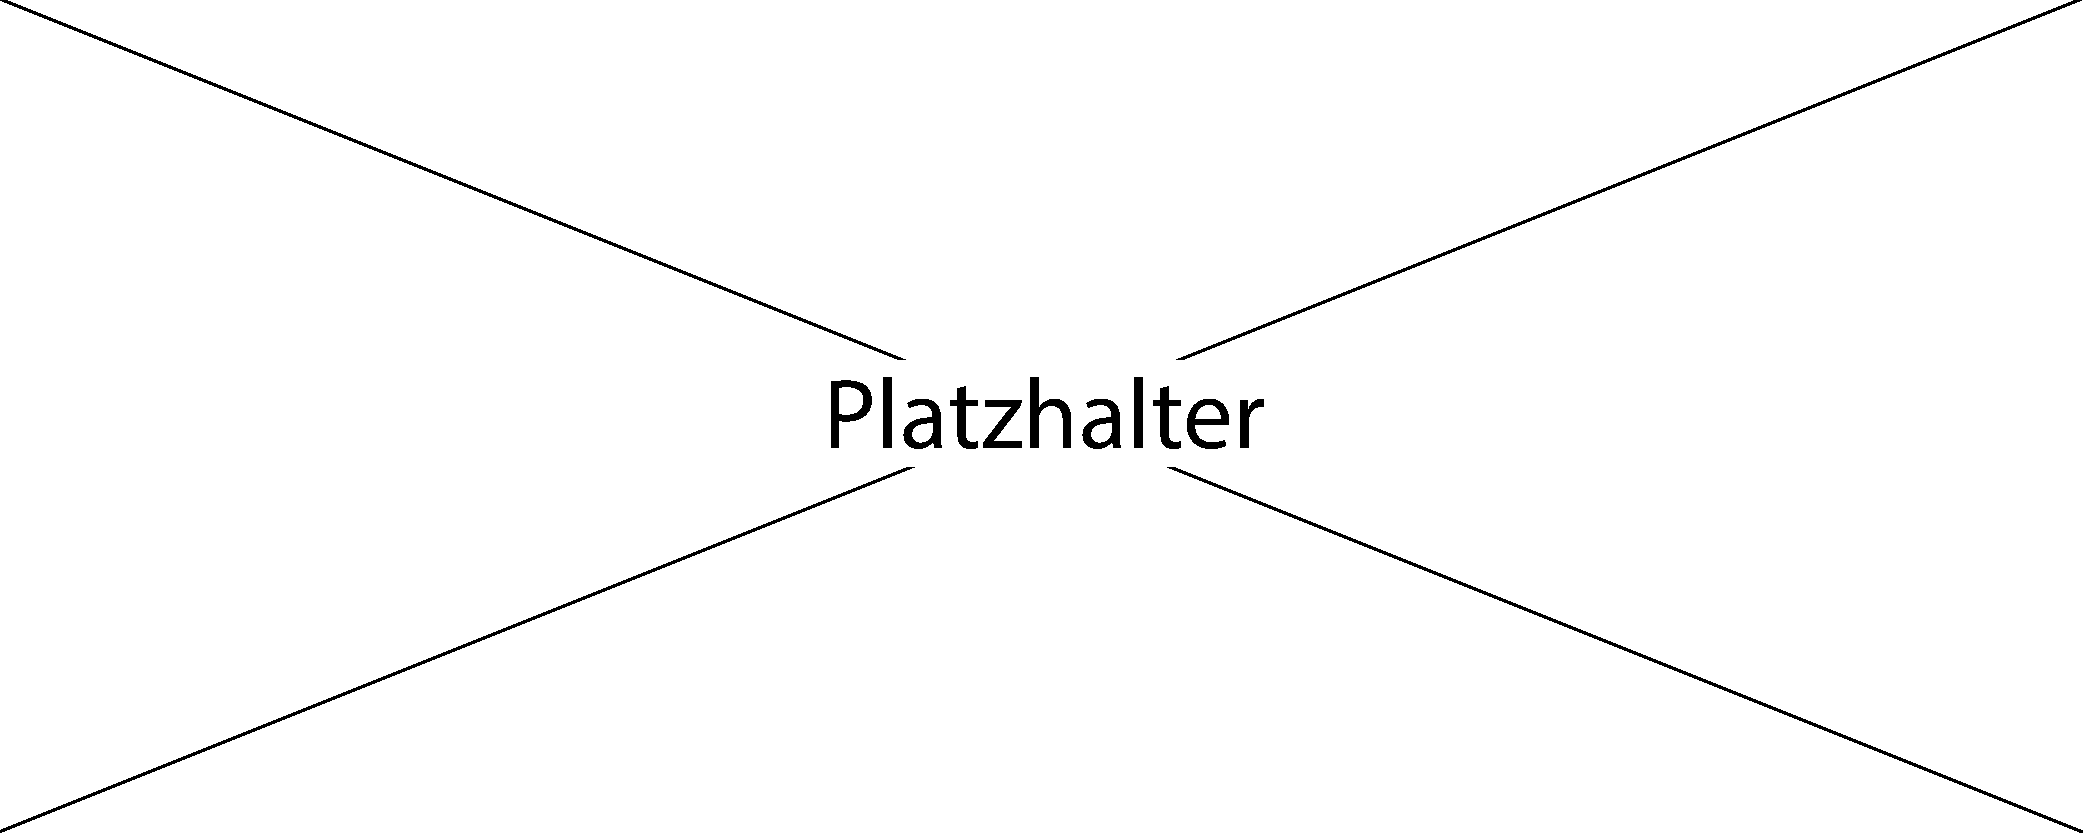
\includegraphics[width=12cm]{figures/sonstiges/platzhalter.pdf}
			\caption{Flowchart des Algorithmus \texttt{RandomSearch}.}
			\label{fig:erg_rs_flow}
		\end{figure}
		Wie darüber hinaus in Abb. \ref{fig:erg_rs_flow} noch einmal verdeutlicht, werden Parameter durch den simplen Input des Rewards variiert und gefunden.\\
		Nach Anwendung der Parametersuche durch \texttt{RandomSearch} wird eine Optimierung des neuronalen Netzes durch \texttt{Weights} durchgeführt. Die gefundenen Parameter sind unter Umständen noch nicht Perfekt gewählt oder verursachen vereinzelt Probleme, welche die Simulation inkonsistent werden lassen. Bei der Optimierung durch Gewichtung der bestehenden Synapsen könnten nachträglich Parameter beeinflusst und gewisse Wege im neuronalen Netz feiner eingestuft werden. In Abb. \ref{fig:erg_w_flow} wird der gesamte Programmablauf noch einmal verdeutlicht.
		\begin{figure}[!h] %[!t] ...
			\centering
			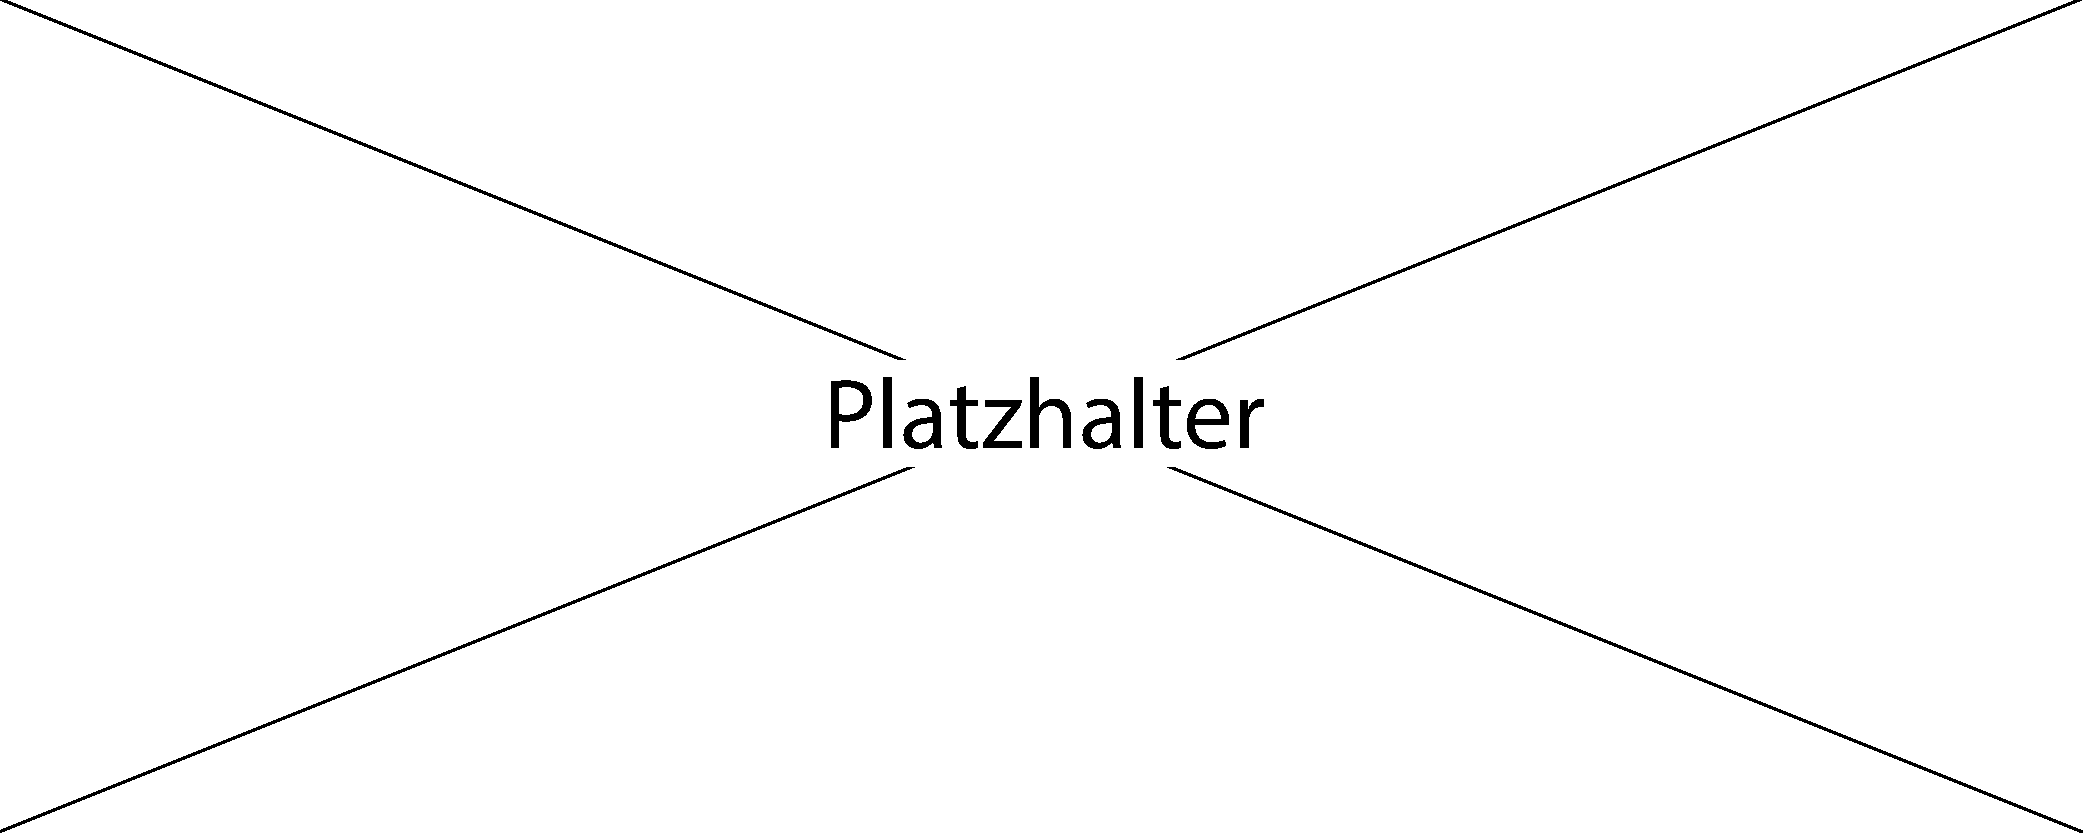
\includegraphics[width=12cm]{figures/sonstiges/platzhalter.pdf}
			\caption{Flowchart des Algorithmus \texttt{Weights}.}
			\label{fig:erg_w_flow}
		\end{figure}
		In Appendix \ref{label} werden die Ergebnisse der besten Simulationsläufe genauer beschrieben.\\
		Eine weitere Optimierung wurde eingeführt, um das neuronale Netz robuster und effizienter zu gestalten. Anstatt der gesamten 46 Parameter für Nervenzellen, Synapsen und Gap-Junctions werden jeweils nur die hälfte der benötigten Parameter simuliert und dupliziert. Dies sorgt für eine symmetrische Verteilung von zufällig generierten Parametern und einer noch effizienteren Simulation. Aufgrund der symmetrischen Architektur des gegebenen neuronalen Netzes ist diese Methode zulässig und führt zu sehr guten Ergebnissen.
	\subsection{Alternative Such- und Optimierungsalgorithmen}
		Wie bereits in Sektion \ref{sec:rl_alt} vorgestellt, existieren bereits viele gute Algorithmen zur Parametersuche und -optimierung von künstlich erzeugten oder gegebenen neuronalen Netzen. Doch die Implementierung dieser Algorithmen besonders auf die hohe Anzahl an zu variierenden Parametern stellt eine hohe Anforderung dar. Klassische Optimierungsverfahren über Kostenfunktionen lassen sich zwar aufstellen (wie in \ref{label}) kurz gezeigt, können aber durch die Anzahl an Nervenzellen, Synapsen und Gap-Junctions nicht weiter optimiert werden.\\
		Einzig die Optimierung durch Gewichtung von Synapsen und Gap-Junctions kann mit bekannten Algorithmen und den Input des Rewards effizienter als durch RandomSearch umgesetzt werden.

% ***
\section{Vergleich zu bestehenden Systemen}
\label{sec:erg_vgl}
% ***
	Vergleich zu bestehenden Systemen aus der Regelungstechnik (nötig?).

% ***
\section{Zusammenfassung}
\label{sec:erg_zsm}
% ***
	

% ***
\section{Ausblick}
\label{sec:erg_ausblick}
% ***

%%% Local Variables: 
%%% mode: latex
%%% TeX-master: "main"
%%% End: 
